\chapter{nome capitlo 1}
\begin{figure}[htbp]
    \centering
    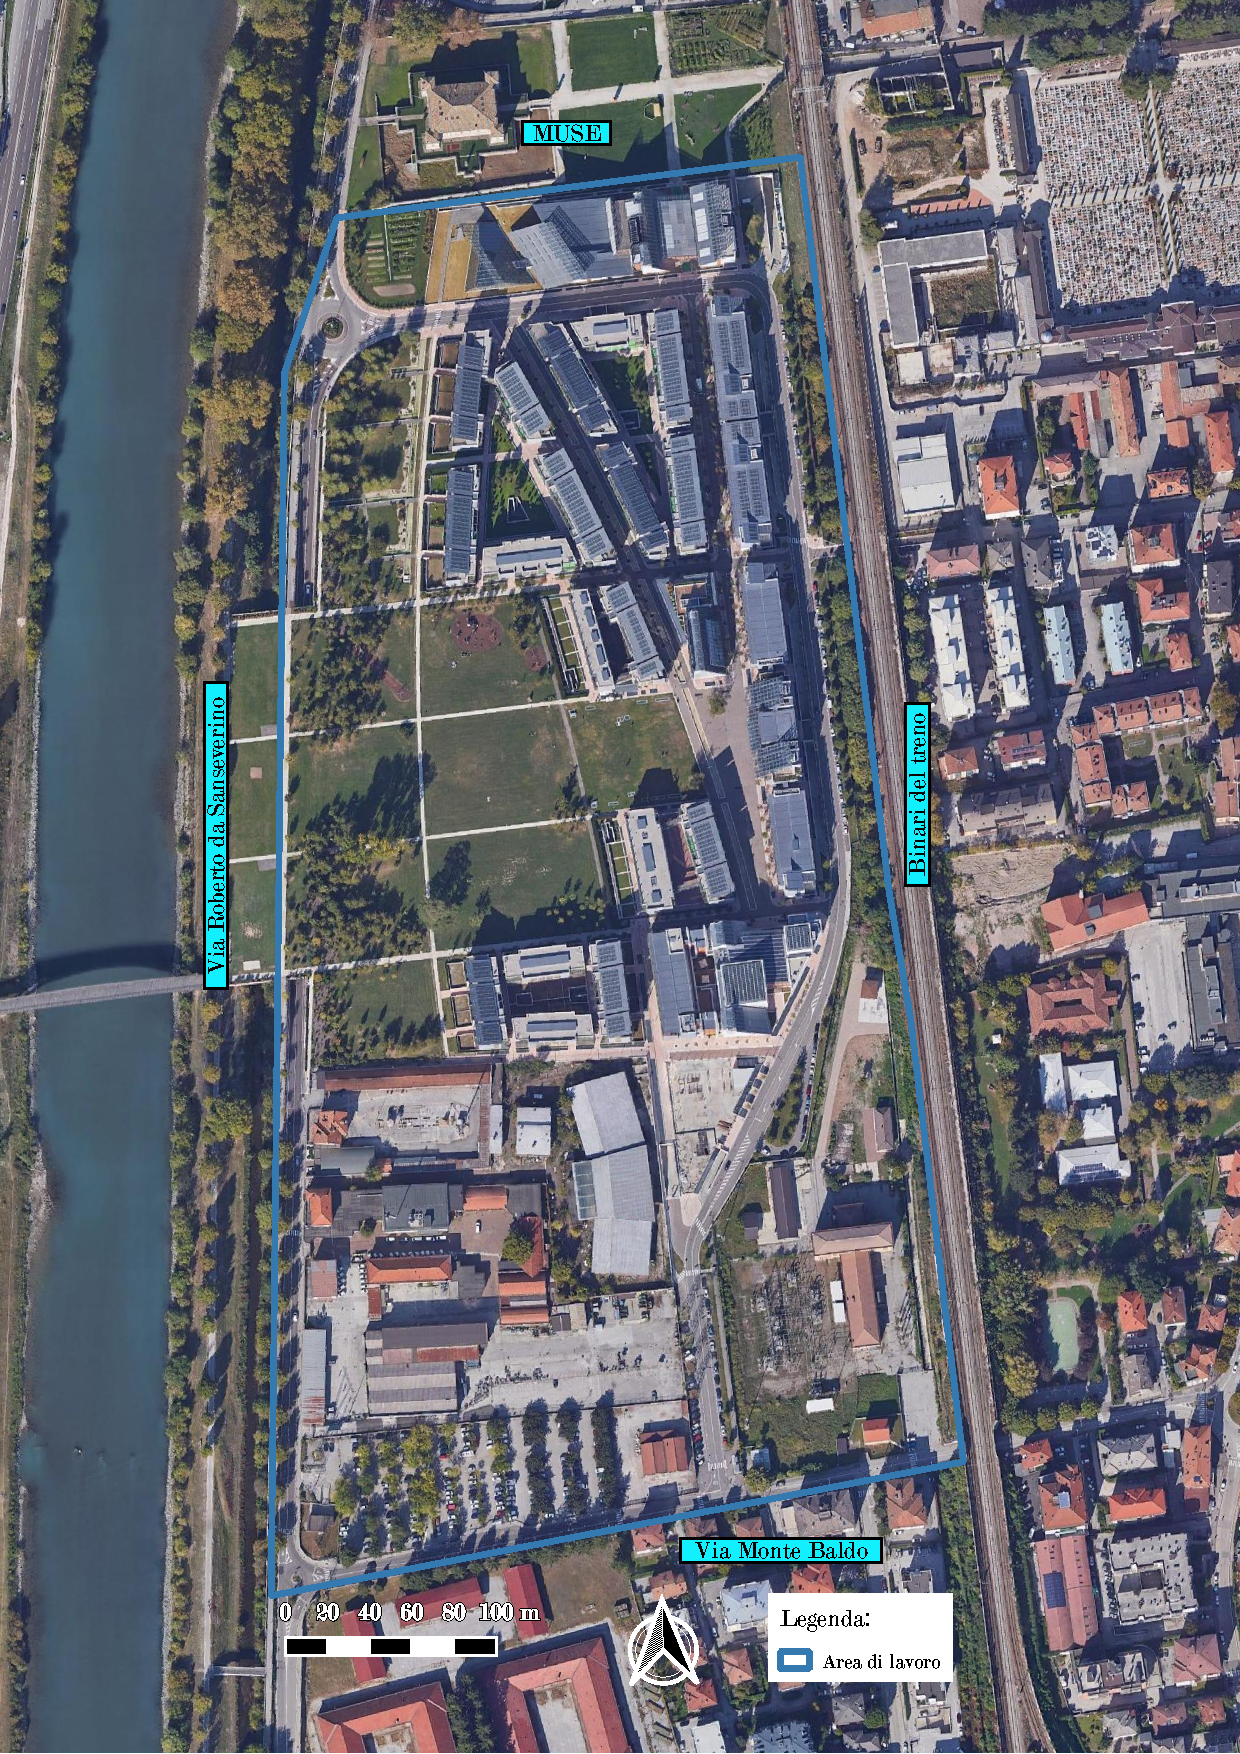
\includegraphics[trim=0cm 0cm 0cm 0cm,clip,frame,width=\textwidth]{IMG/inquadramento.pdf} 
    \caption{Inquadramento dell'area di lavoro}
    \label{fig:inquadramento}
    \end{figure}

\begin{equation}
    i = a \, t_p ^{n - 1}
\end{equation}
\begin{equation}
    CN = \frac{25400}{254 + S}
\end{equation}

\begin{equation}
    T_{\text{dry}} = \frac{3.125}{\sqrt{K_s}}
\end{equation}
Dove $T_{\text{dry}}$ sono i giorni che impiega il suolo completamente saturo a tornare secco e $K_s$ è la conduttività idraulica espressa in \si{inch\per\hour}.
\begin{equation}
    i_m = \frac{h(t_\text{fin}) - h(t_\text{in})}{\Delta t}
\end{equation}
\begin{equation}   
    h(t) = 
    \begin{cases}
        r \, a \left[ \left( \frac{t_p}{r}\right)^n - \left( \frac{t_p - t}{r}\right)^n  \right] & \text{se $t < t_p$}\\
        a \left[ r \left( \frac{t_p}{r}\right)^n + (1-r)\left( \frac{t_p - t}{1 - r}\right)^n  \right] & \text{se $t > t_p$}\\
    \end{cases}
\end{equation}
 


















\begin{landscape}
    \begin{figure}[htb]
        \centering
        \begin{tikzpicture}
            \begin{axis}[
                restrict x to domain=-0:1.5,
                height=15cm,
                width=21cm,
                grid=major,
                xlabel=Tempo trascorso dall'inizio della precipitazione \si{[\hour]},
                ylabel=Deflusso  \si{[\litre\per\second]},
                xtick = {0.5,1,1.5,2,2.5,3,3.5,4},
                %title= ,
                /pgf/number format/.cd,
                use comma,
                1000 sep={\,}
            ]
            \addplot +[mark=none,style=solid,color=red] table[x index=0,y index=1,header=false] {IMG/Total-Inflow/total_inflow_1min.txt};
            \addplot +[mark=none,style=solid,color=green!60!black] table[x index=0,y index=1,header=false] {IMG/Total-Inflow/total_inflow_2min.txt};
            \addplot +[mark=none,style=solid,color=magenta] table[x index=0,y index=1,header=false] {IMG/Total-Inflow/total_inflow_5min.txt};
            \addplot +[mark=none,style=solid,color=cyan] table[x index=0,y index=1,header=false] {IMG/Total-Inflow/total_inflow_10min.txt};
            \addplot +[mark=none,style=solid,color=orange] table[x index=0,y index=1,header=false] {IMG/Total-Inflow/total_inflow_15min.txt};
            \addplot +[mark=none,style=solid,color=teal] table[x index=0,y index=1,header=false] {IMG/Total-Inflow/total_inflow_30min.txt};
            \addplot +[mark=none,style=solid,color=violet] table[x index=0,y index=1,header=false] {IMG/Total-Inflow/total_inflow_45min.txt};
            \legend{1 min,2 min,5 min,10 min,15 min,30 min,45 min}    
            \end{axis}
        \end{tikzpicture}
        \caption{Deflusso del bacino}
        \label{fig:Ietogrammi}
    \end{figure}
\end{landscape}

\begin{landscape}
    \begin{figure}[htb]
        \centering
        \begin{tikzpicture}
            \begin{axis}[
                restrict x to domain=-0:4,
                height=15cm,
                width=21cm,
                grid=major,
                xlabel=Tempo trascorso dall'inizio della precipitazione \si{[\hour]},
                ylabel=Total Inflow  \si{[\litre\per\second]},
                xtick = {0.5,1,1.5,2,2.5,3,3.5,4},
                %title= ,
                /pgf/number format/.cd,
                use comma,
                1000 sep={\,}
            ]
            \addplot +[mark=none,style=solid,color=red] table[x index=0,y index=1,header=false] {IMG/Total-Inflow/total_inflow_5min_Chicago_25anni.txt};
            \end{axis}
        \end{tikzpicture}
        \caption{Andamento dello sforzo assiale agente sul pilastro P27 in funzione dell'altezza}
        \label{fig:IetogrammaFinale}
    \end{figure}   
\end{landscape}